\section{Billedbehandling}
I billedbehandling kan data blive repræsenteret på mange forskellige måder, alt efter hvilket domæne et signal optræder i. To af områderne er f.eks. frekvensdomænet og tid og sted domænet. Man vælger så hvilket domæne der repræsenterer de ønskede karistika i signalet bedst, ved at lave et gæt, eller ved at forsøge sig frem. Har man f.eks. observeret en række målte data, arbejder man typisk med disse i tid og sted domænet, hvor en diskret fouriertranformation producerer information der kan aflæses i frekvensdomænet. 

Når vi ser med menneskeøjne på et billede af en celle, er de som regel uden klart defineret semantik. Da billedet bliver taget som et tværsnit kan vinklen på cellerne være lidt på kanten af en celle der gør at det er svært at se klare overgange mellem cellerne, og kanterne vil i stedet have noget støj der kan gå ud over billedet, hvilket også blev diskuteret i tidligere afsnit.

Fra et datalogisk synpunkt kan vi derfor ønske at transformere dataene i billedet til en mere kompakt repræsentation, hvor vi har lettere tilgængelighed til det semantiske indhold. Man kan forestille sig at vi er interesserede i at fjerne eller nedtone uinteressante detaljer i billedet, såsom denne støj ved cellens kant, eller fremhæve væsentlige ting, som i vores tilfælde med vessiklerne. 

En sådan reduktion af støj, eller ekstraktion af interessante konturer, opnås ved flere skridt af datamatisk analyse. Man kan f.eks se på resultatet efter en filtrering, der typisk er det første skridt i billedbehandling, og se efter kontraster og markant afvigende pletter i forhold til omgivelserne. Disse observationer giver så en indikation af hvilken retning den fortsatte analyse skal gå.

Da man ved filtrering ønsker flere ting, deriblandt både reduktion og ekstraktion, findes der naturligvis mange typer af filtre der kan benyttes i analysen, og det er målet for analysen der bestemmer hvilke filtre der skal benyttes. 

\subsection{Foldning og filtrering}
% Skriv om dette (kantfejl ved foldning)
%http://www.echoview.com/files/WebHelp/Reference/Algorithms/Operators/Convolution_algorithms.htm
Filtreringen foretages ofte ved en foldning af billedet med de valgte filterfunktionener. I matematik og specielt i funktionanalyse, er foldning en matematisk operation på to funktioner, $f$ og $g$, der producerer en tredje funktion der er en modificeret funktion af en af de to funktioner. Foldning opnås ved
\begin{align}
	f(t)*g(t)=\int_{-\infty}^{\infty}f(\tau)g(t-\tau)d\tau
\end{align}
hvor $*$ er tegnet for foldning. 

Man opnår samme resultat ved at folde f og g i tid og sted domænet som man gør ved at multiplicere deres fouriertransformerede i frekvensdomænet, og så invers fouriertransformere.
\begin{align}
	f(t)*g(t) = \mathbb{F}^{-1}(\mathbb{F}(f)\cdot\mathbb{F}(g))
\end{align}
hvor $\mathbb{F}$ betyder at der er foretaget en fouriertransformation af funktionen og $\mathbb{F}^{-1}$ er en invers fouriertransformation.

Når man folder et billede med et filter, besøger man hver pixel og går størrelsen på filteret ud med centrum i denne. I hvert af disse områder beregnes så en værdi som så gemmes i den valgte pixel. På den måde udregner filteret en værdi for hver pixel ved hjælp af de omkringliggende pixels og ikke alle pixels i billedet. Problemet med dette er dog at i kanten af billedet vil filteret på den ene side ikke kunne finde nogle nabopixels. Dette er illustreret grafisk i figur \ref{fig:bildbeh_conv_edge_error}. Her findes så forskellige metoder hvor der kan tages højde for dette. Man kan enten undgå helt at udregne værdier for de pixels der skaber dette problem, eller man kan angive hvilke værdier der skal være i disse pixels. Enten kan man spejle billedet på dets 4 kanter, fortsætte med kantens værdi eller tage den modstående kants værdi. Alle disse metoder er lige korrekte, da ingen af dem bruger sande værdier. 

\begin{figure}[H]
	\centering
	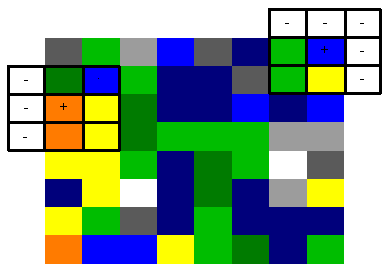
\includegraphics[scale=1]{files/bildbeh/img/conv_edge_error.png}
	\caption{Kantfejl ved foldning.\label{fig:bildbeh_conv_edge_error}}
\end{figure}

Som beskrevet ovenfor er formålet ved en filtrering tit at fremhæve eller dæmpe visse frekvenser som f.eks ved at dæmpe de høje frekvenser og lade de lave passere, eller omvendt, eller at dæmpe nogle udvalgte frekvenser. 

De mest benyttede filtre er de lineære positionsinvariante.\footnote{Forelæsningsnoter til introduktion til billedbehandling, 25. oktober 2006, side 39} Et filter er lineært hvis det kan skrives som et lineært udtryk $O=\mathbf{F}I$ hvor $I$ hhv. $O$ er input hhv. output billeder organiseret som søjlevektorer og $\mathbf{F}$ er en kvadratisk matrix af filterværdier. 

Man kan filtrere billederne i både frekvendomænet og tid og sted domænet. Signaler kan konverteres fra tid og sted domænet til frekvensdomænet, og tilbage igen, gennem fouriertransformation.

\subsubsection{Lav-pas filtrering}
Ved en lav-pas filtrering dæmpes de høje frekvenser og de lave frekvenser får altså lov at passere. Lav-pas filtrering er en effektiv metode til at undertrykke støj, men ulempen er at der sker en reduktion i kontrasten fordi højfrekvent energi fra billedkontraster ikke kan skelnes fra højfrekvent energi fra støj.

Der findes her en række af filtre såsom idealfiltret, Butterworth filtret, Hanning filtret og Gauss filtret. Forskellen i disse filtre er hvordan de efterlader billedet. Da lav-pasfiltret også dæmper de høje frekvensers energi fra billedkontraster kan man f.eks ved idealfiltret opleve ringningseffekt omkring kraftige kontraster i billedet. Butterworth filtret har kun i meget ringe grad ringningseffekt da filtret tillader en portion af høje frekvenser at passere og derfor er "cut-off"-frekvensen glat. Det mest benyttede filter er Gauss filtret.\footnote{Forelæsningsnoter til introduktion til billedbehandling, 25. oktober 2006, side 43}

\subsubsection{Høj-pas filtrering}
Hvor lav-pas filtrering altså dæmpede de høje frekvenser og dermed kontraster og støj, har høj-pas filtrene til formål at fremhæve kontraster ved at dæmpe de lave frekvenser. 

\subsubsection{Bånd-pas filtrering}
Ved en bånd-pas filtrering tillades kun et bestemt frekvensbånd at passere. Passagen kan ske uhindret som i et ideal bånd-pas filter eller dæmpes glat ved overgangen mellem de frekvenser, der passerer, og de, der undertrykkes. Hvis der forekommer meget regelmæssig støj i et billede, vil denne støj optræde som punkter med numerisk stor værdi i styrkespektret for billedet. Det er ofte muligt at se sådanne punkter i et logaritmisk plot af styrkespektret.

\subsection{Tid og sted domænet}
Filtrering i tid og sted domænet foretages med fordel når støtten for filtret er lille, altså når størrelsen på filteret der foldes med er lille. Fordelen ved filtrering i tid og sted domænet bliver særlig stor hvis filtret er separabelt. 

Hvis filtreringens formål er at fjerne støjen, og støtten for filtret er stor, vil filtrets egenskab mht. undertrykkelse af støj som regel være god. Generelt er det nødvendigt at øge støtten jo ringere signal-støjforholdet i et billede er. Signal-støjforholdet er defineret ved forholdet mellem energien i signalet og energien i støjen. Hvis filtreringens formål er at producere et billede til efterfølgende menneskelig inspektion, vil det imidlertid ofte ære en fordel at holde støtten lille.

To meget benyttede filtre er box filtret og Gauss filtret. En egenskab ved Gauss filtret er at dette filter vil fremkomme ved gentagende filtrering af et vilkårligt filter med sig selv.\footnote{Forelæsningsnoter til introduktion til billedbehandling, 25. oktober 2006, side 46}

\subsection{Frekvensområdet}
Hvor tid og sted domænet f.eks. viser grafer over hvordan signalet ændrer sig over tid, viser grafen i frekvensområdet i stedet hvor meget af signalet der ligger inden for en række frekvenser der danner et bånd. I frekvensområdet arbejder man med fouriertranformationer.

\subsubsection{Fouriertransformation}
Fouriertransformation kommer fra studierne i Fourierserier, der er en måde at dekomposere et hvilken som helst periodisk signal til summen af et sæt af simple svingende funktioner, f.eks sinus og cosinus. Fourierserier blev introduceret af Joseph Fourier (1768-1830) med formålet at løse varmeligningen i en metalplade.

Navnet Fouriertransformation refererer både til frekvensdomænet af signalet og processen der transformerer signalet til dets frekvensdomænerepræsentation. Fouriertransformation er klassisk inden for al signal- og billedbehandling. Dette skyldes bl.a. at en række foldninger kan beregnes væsentlig hurtigere ved brug af fouriertransformationen. Fouriertransformationen giver mulighed for visuelt at fortolke billedet på en ny måde og for at specificere visse filtre lettere. Matematisk set er fouriertransformationen blot en ud af mange baseskiftende transformationer.

% SKRIV MERE MATEMATISK HVAD FOURIERTRANSFORMATION ER.

% VIS EKSEMPLER PÅ BILLEDER I FOURIER OMRÅDER OG VIS SKRIDTERE GRAFISK

%% Referencer:
% http://en.wikipedia.org/w/index.php?title=Digital_signal_processing&oldid=426007207
% http://en.wikipedia.org/w/index.php?title=Frequency_domain&oldid=424506778
% Forelæsningsnoter til introduktion til billedbehandling, 25. oktober 2006
